% Generated from the public primitive catalog. Original Atlas drawing; Apache-2.0.
% Target: aes-dm-128; view: overview
\documentclass[border=9pt]{standalone}
% Original Atlas figure theme. Apache-2.0; see the repository LICENSE.
\usepackage[T1]{fontenc}
\usepackage{lmodern}
\usepackage{amsmath,amssymb}
\usepackage{tikz}
\usetikzlibrary{arrows.meta,positioning,calc,fit,backgrounds,decorations.pathreplacing,matrix}
\definecolor{atlasInk}{HTML}{172235}
\definecolor{atlasTeal}{HTML}{0D7B7D}
\definecolor{atlasMuted}{HTML}{637278}
\definecolor{atlasFill}{HTML}{EAF4F2}
\definecolor{atlasLine}{HTML}{B6C8C7}
\tikzset{
  every picture/.style={line width=.65pt,draw=atlasInk,>=Latex},
  every node/.style={text=atlasInk,font=\sffamily\small},
  box/.style={draw,rounded corners=1.5pt,minimum height=.9cm,minimum width=1.6cm,align=center,inner sep=6pt,fill=white},
  accent/.style={box,draw=atlasTeal,fill=atlasFill},
  wire/.style={->,line width=.7pt},
  keywire/.style={wire,draw=atlasTeal,dashed},
  xor/.style={draw,circle,fill=white,inner sep=0pt,minimum size=.38cm},
  add/.style={draw,rectangle,fill=white,inner sep=0pt,minimum size=.38cm},
  note/.style={font=\sffamily\scriptsize,text=atlasMuted,align=center},
  phase/.style={font=\sffamily\small\bfseries,text=atlasTeal},
  group/.style={draw=atlasLine,dashed,rounded corners=2pt,inner sep=8pt}
}
\newcommand{\rotl}{\mathbin{\lll}}
\newcommand{\rotr}{\mathbin{\ggg}}
\newcommand{\kx}{\operatorname{Keccak}\!\text{-}\!f[1600]}

\newcommand{\AtlasCompressionKey}{m}
\newcommand{\AtlasCompressionData}{h}
\newcommand{\AtlasCompressionKeyBits}{128}
\newcommand{\AtlasCompressionDataBits}{128}
\newcommand{\AtlasCompressionOutputBits}{128}
\newcommand{\AtlasCompressionRounds}{10}
\newcommand{\AtlasCompressionMP}{0}
\newcommand{\AtlasCompressionFormula}{F(h,m)=\operatorname{AES}_{m}(h)\oplus h}
\begin{document}
% Original Atlas compression-construction diagram. Apache-2.0.
% CGLSZ25, Section 2.2, Figure 2. Not an iterated hash or an attack diagram.
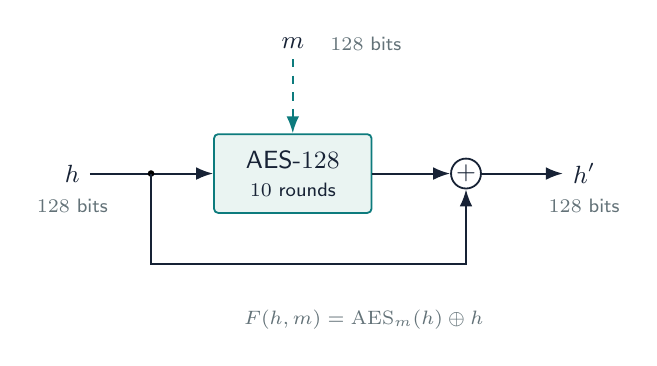
\begin{tikzpicture}
  \node (input) at (0,0) {$\AtlasCompressionData$};
  \node[note,anchor=north] at (0,-.2) {$\AtlasCompressionDataBits$ bits};
  \node[accent,minimum width=2cm,minimum height=1cm] (aes) at (2.8,0)
    {AES-$\AtlasCompressionKeyBits$\\[-1pt]{\scriptsize $\AtlasCompressionRounds$ rounds}};
  \node (key) at (2.8,1.65) {$\AtlasCompressionKey$};
  \node[note,anchor=west] at (3.15,1.65) {$\AtlasCompressionKeyBits$ bits};
  \draw[keywire] (key) -- (aes);
  \node[xor] (feed) at (5,0) {$+$};
  \draw[wire] (input) -- (aes);
  \draw[wire] (aes) -- (feed);
  \fill (1,0) circle (1.2pt);
  \draw[wire] (1,0) -- (1,-1.15) -- (5,-1.15) -- (feed.south);
  \ifnum\AtlasCompressionMP=1
    \node[xor] (extra) at (6.3,0) {$+$};
    \draw[wire] (feed) -- (extra);
    \fill[atlasTeal] (2.8,1.15) circle (1.2pt);
    \draw[wire,draw=atlasTeal] (2.8,1.15) -- (6.3,1.15) -- (extra.north);
    \node (out) at (7.6,0) {$h'$};
    \draw[wire] (extra) -- (out);
    \node[note,anchor=north] at (7.6,-.2) {$\AtlasCompressionOutputBits$ bits};
  \else
    \node (out) at (6.5,0) {$h'$};
    \draw[wire] (feed) -- (out);
    \node[note,anchor=north] at (6.5,-.2) {$\AtlasCompressionOutputBits$ bits};
  \fi
  \node[note] at (3.7,-1.85) {$\AtlasCompressionFormula$};
\end{tikzpicture}

\end{document}
